\chapter{Quickstart Example}\label{chp:Quickstart-Example}

	As an exemplaric application to demonstrate the monitoring and analysis within \Kieker{}, we introduce the Bookstore application. It is a small sample application resembling a simple bookstore with a market-place facility where users can search for books in an online catalog, and subsequently get offers from different book sellers. The example without any monitoring or analysis code can be found in \dir{\plainBookstoreApplicationDirDistro}. The instrumented bookstore can be found in \dir{\quickstartBookstoreApplicationDirDistro}.

	\section{Monitoring}
	
		Before we can start with the actual instrumentation, we have to compile our example.
		\setBashListing
		\begin{lstlisting}[gobble=6,caption=]
			#\lstshellprompt{}# mkdir build
			#\lstshellprompt{}# javac src/kieker/examples/userguide/ch2bookstore/*.java -d build/
		\end{lstlisting} 

		\noindent
		After setting up the example, we use AspectJ \cite{AspectJ-WebSite} to weave the \Kieker{} monitoring code into the Bookstore application during runtime. It is necessary to perform the following steps:
		\begin{enumerate}
			\setlength{\itemsep}{-2pt}
			\item Instruct AspectJ to weave \Kieker{}'s monitoring code into the application
			\item Configure \Kieker{} to write the monitoring logs to the file system
			\item Start the Bookstore application with Aspectj as a so called Java-Agent 
		\end{enumerate}
	
		\noindent
		For the first two steps, we copy the \dir{META-INF} folder from the root directory into the \dir{build} directory. This folder contains the necessary configuration files for both AspectJ and \Kieker{}. Additionally we have to copy the \file{dist/\mainJarWeaver} into a new \dir{lib} directory in the directory of the bookstore example. This jar file contains not only \Kieker{}, but AspectJ as well. For the third step we can use the following command.
		
		\setBashListing
		\begin{lstlisting}[gobble=6,caption=]			
			#\lstshellprompt{}# java -javaagent:lib/#\mainJarWeaver# -classpath build
			    kieker.examples.userguide.ch2bookstore.BookstoreStarter
		\end{lstlisting} 
		
		\noindent
		By executing the instrumented example, \Kieker{} produces monitoring data (e.g., in a folder \dir{kieker-20140224-152329453-UTC-Laptop-KIEKER}), which can be found in the system's temporary folder.
	
	\section{Analysis}
	
		After we have created some monitoring logs, we use our Trace Analysis Tool to visualize the results. In order to use this tool, we have to install Graphviz (\url{http://www.graphviz.org}) first and add it to your system's path. \\

		\NOTIFYBOX{The Trace Analysis Tool is just one way to process monitoring data. It is of course always possible to use self-defined analyses. We show this in Chapter~\ref{chp:Kieker-Analysis}. Furthermore, the whole potential of the Trace Analysis Tool is detailed in Chapter~\ref{chp:Kieker-Tools}.}
		
		\noindent
		Our Trace Analysis Tool can be used to generate various graphs. However, we will generate only two of these graphs: A call tree and a component overview. We use the script \file{trace-analysis.sh|bat} which can be found in the \dir{bin} directory of the release. We create a folder named \dir{out} in the \dir{bin} directory and use the following command to generate the graphs (the input directory has of course to be adjusted in order to match the directory with the monitoring log created in the previous section).
		
		\setBashListing
		\begin{lstlisting}[gobble=6,caption=]			
			#\lstshellprompt{}# trace-analysis.sh -i /tmp/kieker-20140224-152329453-UTC-Laptop-KIEKER -o out 
			    --plot-Aggregated-Assembly-Call-Tree  --plot-Assembly-Component-Dependency-Graph
		\end{lstlisting} 
		
		\noindent
		The results are two \file{.dot} files in the \dir{out} directory. They can be converted using the script \file{dotPic-fileConverter.sh|bat} (which is just a wrapper for the Graphviz tool).
		
		\setBashListing
		\begin{lstlisting}[gobble=6,caption=]			
			#\lstshellprompt{}# dotPic-fileConverter.sh out png
		\end{lstlisting} 
		
		\noindent
		Now, we have two \file{.png} files in the \dir{out} directory, each containing a different visual representation of the monitoring.		
		
		\begin{figure}[H]
			\centering
			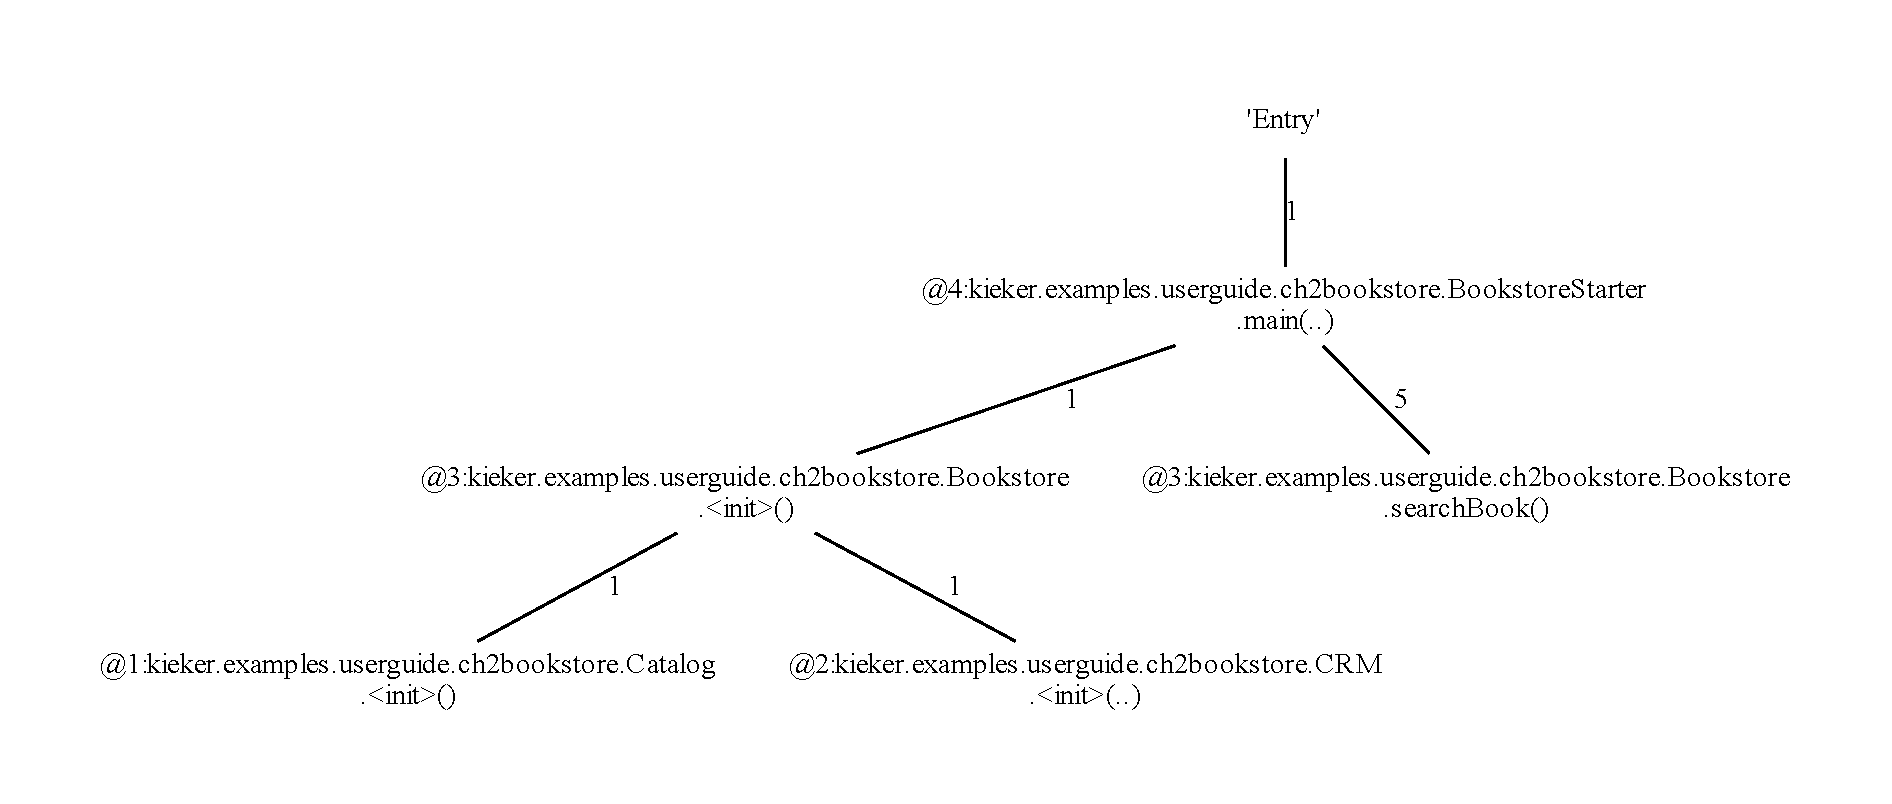
\includegraphics[width=0.8\textwidth]{images/aggregatedAssemblyCallTree.pdf}
		\end{figure}
		\begin{figure}[H]
			\centering
			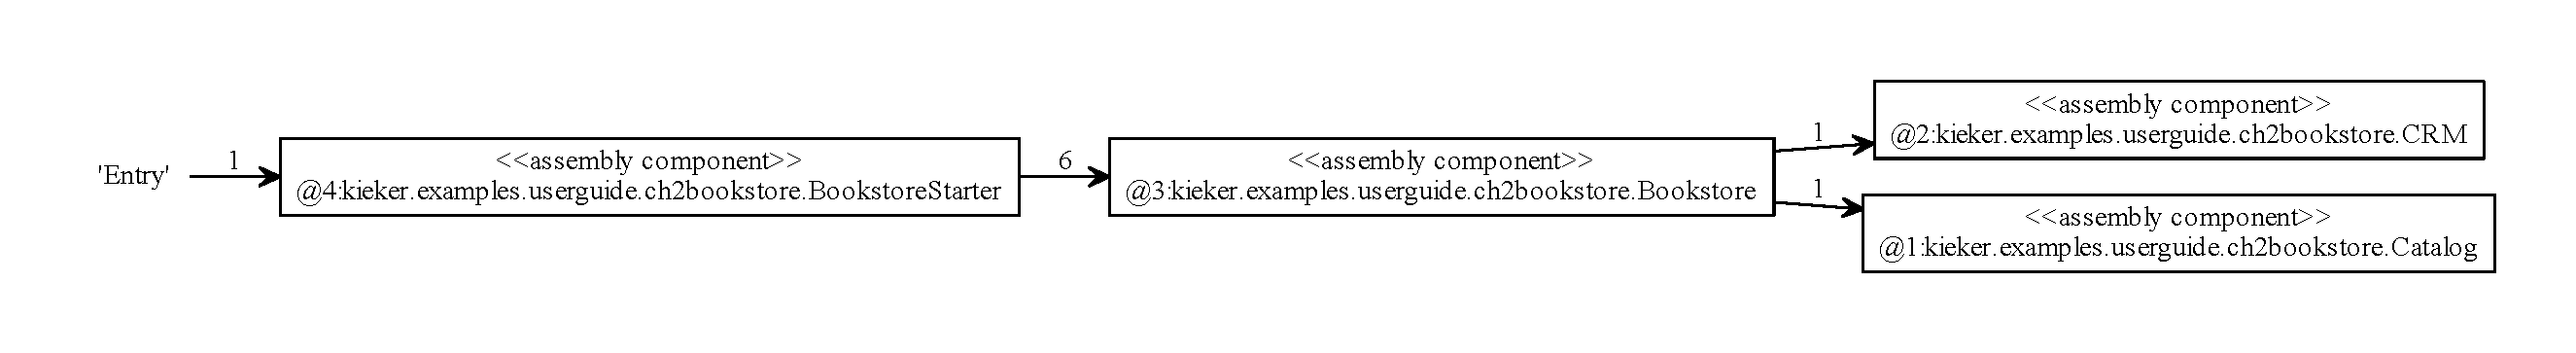
\includegraphics[width=1.0\textwidth]{images/assemblyComponentDependencyGraph.pdf}
		\end{figure}